\documentclass{beamer}
\usepackage[utf8]{inputenc}
\usepackage[spanish]{babel}
\usepackage{tikz}
\usepackage{amsmath}
\usepackage{graphicx} 
\usetheme{Madrid}       % bordes, header y footer
\usecolortheme{default} % colores
\usetikzlibrary{shapes.geometric, arrows, positioning, trees, calc, backgrounds, fit}

% Configuración de Estilos TikZ
\tikzstyle{box} = [rectangle, rounded corners, minimum width=2cm, minimum height=0.8cm, text centered, draw=black, fill=blue!10]
\tikzstyle{arrow} = [thick,->,>=stealth]
\tikzstyle{decision} = [diamond, minimum width=2cm, minimum height=1cm, text centered, draw=black, fill=green!10]

\title{Shadow Symbolic Execution: Verificación Dinámica de Parches}
\subtitle{Testing for Divergences Between Software Versions}
\author{Hristina Palikareva, Tomasz Kuchta, Cristian Cadar}
\institute{Imperial College London}
\date{ICSE 2016}

\begin{document}

\begin{frame}
\titlepage
\end{frame}

%% 1. Motivación: El Problema del Patch Testing
\begin{frame}{Motivación: El Problema del Patch Testing}
\begin{itemize}
    \item Los cambios en el software suelen introducir errores y vulnerabilidades.
    \item La cobertura de lineas es insuficiente: se puede cubrir un parche sin ejecutar el \textbf{nuevo comportamiento} introducido.
    \item \textbf{Limitación actual:} Los casos de prueba a menudo ejercitan el mismo comportamiento en ambas versiones.
    \item \textbf{Solución:} Generar entradas que fuercen la divergencia entre la versión antigua y la nueva.
\end{itemize}
\end{frame}


\begin{frame}{Cobertura 100\% ...}
\centering

\begin{tikzpicture}[scale=1, every node/.style={font=\small}]

  % Recta numérica más larga para dar espacio
  \draw[<->, thick] (-0.5,0) -- (11.5,0);

  % Ticks en posiciones más separadas: 0, 2.5, 5, 7.5, 10
  \foreach \x/\lbl in {0/0, 2.5/10, 5/20, 7.5/30, 10/40} {
    \draw (\x, 0.1) -- (\x, -0.1);
    \node[below] at (\x, -0.15) {\lbl};
  }

  % Punto ciego entre 10 y 20 (x=2.5 a x=5)
  \filldraw[fill=orange!70!black, draw=orange!80!black, rounded corners=3pt]
    (2.5, 0.15) rectangle (5, 0.75);
  \node[white, font=\scriptsize\bfseries] at (3.75, 0.45) {PUNTO CIEGO};

  % Checkmarks
  \node[green!50!black, font=\large] at (0, 0.65) {$\checkmark$};
  \node[green!50!black, font=\scriptsize, above] at (0, 0.75) {\texttt{x = 0}};

  \node[green!50!black, font=\large] at (7.5, 0.65) {$\checkmark$};
  \node[green!50!black, font=\scriptsize, above] at (7.5, 0.75) {\texttt{x = 30}};

  % Flechas punteadas
  \draw[->, dashed, gray] (2.5, -1.8) -- (2.5, -0.6)
  ;
  \draw[->,  dashed, gray] (5,   -1.8) -- (5,   -0.6);

  % Caja versión antigua — centrada en x=2.5
  \node[draw=teal!60!black, fill=teal!10, rounded corners=4pt,
        minimum width=3cm, minimum height=0.7cm,
        font=\ttfamily\small] at (2.5, -2.3) {if (x > 10)};
  \node[font=\tiny, text=teal!60!black] at (2.5, -2.9) {versión antigua};

  % Caja versión nueva — centrada en x=5
  \node[draw=orange!70!black, fill=orange!10, rounded corners=4pt,
        minimum width=3cm, minimum height=0.7cm,
        font=\ttfamily\small] at (6, -2.3) {if (x > 20)};
  \node[font=\tiny, text=orange!70!black] at (5, -2.9) {versión nueva};

\end{tikzpicture}

\vspace{0.5em}
{\color{black}
  Tests con \texttt{x=0} y \texttt{x=30} logran cobertura total en ambas versiones, pero los valores que generan divergencias (11--20) jamás se evalúan.
}

\end{frame}

%% 3. Shadow Intro
\begin{frame}{Shadow}
\begin{itemize}
  \item \textbf{¿Qué hace?}
  \begin{itemize}
    \item Ejecuta ambas versiones en la misma instancia de Ejecución Simbólica.
    \item Determina precisamente cuando hay divergencia en el comportamiento
    \item Tiempo de ejecución y consumo de memoria bajos
  \end{itemize}
  \item \textbf{¿Cómo lo hace?}
  \begin{enumerate}
    \item Unifica ambas versiones usando anotaciones \texttt{change()}.
    \item Selecciona casos de prueba que ejecuten el parche.
    \item Symbolic Execution con bifurcación de cuatro vías para detectar divergencias.
    \item Re-ejecución nativa para validar divergencias y clasificar resultados.
  \end{enumerate}
\end{itemize}
  \end{frame}


%% 4. Flow de Trabajo de Shadow
\begin{frame}{Flujo de Trabajo de SHADOW}
\centering
\begin{tikzpicture}[node distance=1cm, scale=0.6, every node/.style={scale=0.6}]
    \node (old) [box] {Versión Antigua};
    \node (new) [box, right=of old] {Versión Nueva};
    \node (unify) [box, below=0.8cm of $(old)!0.5!(new)$] {Unificar (change() annotations)};
    \node (select) [box, below=of unify] {Selección: Test que tocan el parche};
    % Dos fases internas
    \node (concolic) [box, fill=orange!40, below=0.9cm of select, xshift=-1.34cm, minimum width=2.2cm, minimum height=0.8cm] {1. Concolic Phase};
    \node (bse)      [box, fill=orange!20, right=0.3cm of concolic, minimum width=2.2cm, minimum height=0.8cm] {2. BSE};
    % Contenedor con borde negro
    \begin{pgfonlayer}{background}
        \node [draw=black, fill=orange!10, rounded corners=6pt, thin,
               fit=(concolic)(bse), inner xsep=1.3cm, inner ysep=0.8cm] (symexec) {};
    \end{pgfonlayer}
    % Etiqueta anclada al borde superior del contenedor
    \node [font=\small\bfseries, anchor=north] at (symexec.north) {Shadow Symbolic Execution};

    \node (replay) [box, below=0.8cm of symexec] {Cross-version Checks (Native Replay)};
    \node (bugs) [box, fill=red!20, below left=0.8cm and 1.2cm of replay] {Bugs de Regresión};
    \node (diverg) [box, fill=yellow!20, below right=0.8cm and 1.2cm of replay] {Divergencias Esperadas};

    \draw [arrow] (old) -- (unify); \draw [arrow] (new) -- (unify);
    \draw [arrow] (unify) -- (select); \draw [arrow] (select) -- (symexec);
    \draw [arrow] (symexec) -- (replay);
    \draw [arrow] (replay) -- (bugs);
    \draw [arrow] (replay) -- (diverg);
\end{tikzpicture}
\end{frame}


% 5. Paso 1: Unificación de Versiones
\begin{frame}{1. Unificación de Versiones: El Macro \texttt{change()}}
\begin{itemize}
    \item Las versiones se ejecutan en \textbf{lockstep} (sincronía) hasta divergir.
    \item \textbf{Patrones de Anotación:}
    \begin{itemize}
        \item \textbf{Rvalues:} \texttt{x = change(E1, E2)}
        \item \textbf{Condicionales:} \texttt{if (A \&\& change(true, B))} para fortalecer condiciones.
        \item \textbf{Código Lineal:} \texttt{if (change(true, false)) \{ old\_code \}} para eliminar fragmentos.
    \end{itemize}
\end{itemize}

\begin{figure}
  \centering
  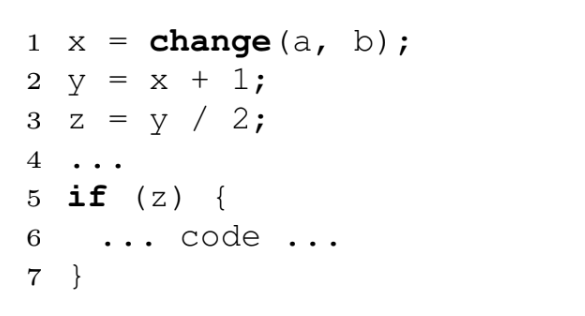
\includegraphics[width=0.6\textwidth]{images/change.png}
  \caption{Ejemplo de uso de \texttt{change()} para unificar código}
\end{figure}
\end{frame}


\begin{frame}{2. Fase de Ejecución Simbólica Shadow}
  \begin{itemize}
    \item \textbf{1. Concolic Phase:} Ejecuta la entrada inicial, y recopila puntos de divergencia.
    \begin{itemize}
      \item Computacionalmente muy barato.
      \item Explora solo el camino concreto, pero detecta divergencias potenciales.
    \end{itemize}
    \item \textbf{2. Bounded Symbolic Execution (BSE):} Para cada punto de divergencia, se ejecuta una BFS solo en la versión nueva. 
    \begin{itemize}
      \item Permite explorar el comportamiento divergente y su impacto sistemáticamente.
    \end{itemize}
\end{itemize}
\end{frame}


\begin{frame}{2.1 Concolic Phase: Four-way Forking}
\centering
\begin{tikzpicture}[level distance=1.2cm,
  level 1/.style={sibling distance=2.5cm},
  level 2/.style={sibling distance=1.2cm},
  scale=0.7, every node/.style={scale=0.7}]
  
  \node [circle, draw] {Branch}
    child {node [rectangle, draw] {$new \land old$}
      child {node {Same Path}}
    }
    child {node [rectangle, draw, fill=gray!30] {$new \land \neg old$}
      child {node {Diff}}
    }
    child {node [rectangle, draw, fill=gray!30] {$\neg new \land old$}
      child {node {Diff}}
    }
    child {node [rectangle, draw] {$\neg new \land \neg old$}
      child {node {Same Path}}
    };
\end{tikzpicture}
\vspace{5pt}

\raggedright
A medida que el programa ejecuta, cada vez que se encuentra una bifurcación (branch), se definen 2 casos:
    \begin{itemize}
        \item \textbf{Diff:} Las versiones divergen en este punto. Se detiene la ejecución sombra, y se encola el punto para exploración posterior en la fase 2.
        \item \textbf{Same Path:} Ambas versiones siguen el mismo camino, pero una divergencia es posible. Se genera un caso de prueba que ejecute esa diferencia, se encola para la fase 2. Se continúa la ejecución concolic.
    \end{itemize}
\end{frame}

\begin{frame}{2.2 Bounded Symbolic Execution (BSE)}
\centering
\begin{tikzpicture}[sibling distance=1.5cm, level distance=1cm, 
    every node/.style={circle, draw, minimum size=0.6cm}, scale=0.8]
    \node {z}
        child {node {y}
            child {node [rectangle, fill=yellow!20, minimum width=1.5cm] {DIFF}
                child {node {a}}
                child {node {b}}
            }
            child {node {1}}
        }
        child {node {2}};
\end{tikzpicture}
\begin{itemize}
    \item Sobre cada punto de divergencia encontrado, se ejecuta una Bounded Symbolic Execution \textbf{solo en la versión nueva}.
    \item \textbf{Ventajas:} Permite generar otros inputs divergentes que muestren el mismo comportamiento de branching hasta ese punto, pero fistinto luego. 
\end{itemize}
\end{frame}

\begin{frame}{Expresiones Shadow}

Los parches normalmente afectan un subconjunto pequeño de expresiones simbólicas, por lo que se introducen \textbf{expresiones shadow} para representar el estado de ambas versiones sin duplicar toda la información.
\begin{figure}
  \centering
  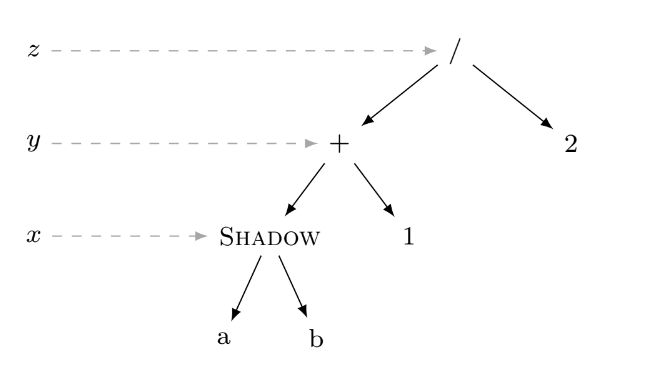
\includegraphics[width=0.6\textwidth]{images/shadow_exp.png}
  \caption{Árbol de expresiones compartido para las variables x, y y z. 
  Las expresiones que contienen subexpresiones shadow se mantienen en el almacenamiento
  simbólico y se evalúan de forma lazy en los puntos de bifurcación.}
\end{figure}
\end{frame}

\begin{frame}{3. Cross-version Checks}
Se busca determinar si uni input divergente realmente expone un bug o es una divergencia esperada.  
\begin{itemize}
    \item \textbf{Cross-version Checks:} Se corren ambas versiones de forma natica con el input divergente generado, y se comparan los outputs y exit codes.
    \item \textbf{Detección de Errores Genéricos:} Se utiliza \textbf{AddressSanitizer} para identificar\textit{buffer overflows}o \textit{crashes}. 
    \item \textbf{Clasificación:}
    \begin{itemize}
        \item Bug de regresión si la nueva falla y la antigua no.
        \item Divergencia esperada si el cambio es intencional según el commit (requiere de análisis humano a veces).
    \end{itemize}
\end{itemize}
\end{frame}

\begin{frame}{Resultados: Victorias de SHADOW}
\begin{enumerate}
    \item \textbf{Bugs reales encontrados:} buffer overflow en \texttt{cut} (patch \#6) y un bug adicional en patch \#21 no cubierto por el test suite original.
    \item \textbf{Four-way forking eficiente:} consumo de memoria nunca superó los 2\,GB por invocación gracias a las \textit{shadow expressions}.
    \item \textbf{Inputs para documentación:} generó divergencias esperadas útiles para agregar al test suite de regresión.
    \item \textbf{Escala a patches grandes:} anotó patches de hasta cientos de LOC; el esfuerzo crece con hunks, no con tamaño.
\end{enumerate}
\end{frame}

\begin{frame}{Resultados: Limitaciones de SHADOW}
\begin{enumerate}
    \item \textbf{Anotaciones manuales:} el pipeline depende de unificar versiones a mano con \texttt{change()}, lo que es error-prone y no escala.
    \item \textbf{Hereda limitaciones de KLEE:} sin soporte para punto flotante, directorios simbólicos ni permisos de archivos, bugs \#1, \#8 y \#14 no detectados.
    \item \textbf{Demasiadas divergencias:} patch \#21 genera $>$21.000 divergencias sin ranking ni clustering para priorizarlas.
    \item \textbf{Solo flujo de control:} cambios en propiedades no funcionales (memoria, performance) son invisibles para la técnica.
    \begin{itemize}
        \item Ejemplo: \texttt{int f(int a, int b) \{...; return a - b;\}}, patch: \texttt{return a - b} $\to$ \texttt{return a + b}. No hay divergencia de control, pero el comportamiento es completamente diferente.
    \end{itemize}
\end{enumerate}
\end{frame}

\end{document}
